\section*{Zadanie 22.}
\begin{task}
\begin{enumerate}[a)]
\item Wymienić ogólne własności fal w liniach TEM.
\item Wymienić praktycznie stosowane typy linii TEM. Dla każdego typu naszkicować rozkład pola \textsl{E} i \textsl{H} w przekroju poprzecznym linii. Podać ich cechy charakterystyczne, jak np: poziom impedancji charakterystycznej, odporność na zakłócenia, koszt i powtarzalność wykonania, elastyczność w wykonywaniu różnych obwodów w.cz., stałość parametrów w funkcji częstotliwości oraz wynikające z tych cech zakresy zastosowań.
\item Obliczyć pojemność rozwartego odcinka 1 m powietrznej linii współosiowej o impedancji charakterystycznej 50 $\Omega$ (przy założeniu, że długość fali jest dużo większa niż 1 m).\\
\end{enumerate}
\end{task}

\begin{solution}
Cechy fali TEM:
\begin{itemize}
\item brak składowych pól elektrycznego i magnetycznego wzdłuż kierunku rozchodzenia się fali,
\item jest to fala poprzeczna
\item w płaszczyźnie $\perp $ do kierunku rozchodzenia się fali pole elektryczne jest bezwirowe
\item prądy płyną w kierunku rozchodzenia się fali i są jednoznacznie określone
\item moc liczona liniowo (z wektora Poyntinga) i obwodowo ($IU$) dają takie same wyniki
\item $Z_{CH}=Z_{f}$
\item $Z,\ L,\ C$ liczone ze wzorów liniowych i obwodowych dają te same wyniki.
\end{itemize}
W liniach TEM operatory z równań Maxwella rozdzielają się na część poprzeczną i wzdłużną $\nabla=\nabla_{\perp}+\nabla_{\parallel}$
$$(\nabla_{\perp}+\nabla_{\parallel})\times\vec{H_{\perp}}=(\sigma + j\omega\epsilon)\vec{E_{\perp}}
\implies \nabla_{\perp}\times\vec{H_{\perp}}=0 \ \ \ \nabla_{\parallel}\times\vec{H}=(\sigma+j\omega\epsilon)\vec{E_{\perp}}$$

$$(\nabla_{\perp}+\nabla_{\parallel})\times\vec{E_{\perp}}=j\omega\mu\vec{H_{\perp}}
\implies \nabla_{\perp}\times\vec{E_{\perp}}=0 \ \ \ \nabla_{\parallel}\times\vec{E}=j\omega\mu\vec{H_{\perp}}$$
Cechy linii TEM:
\begin{itemize}
\item przekrój niezmienny względem $Oz$,
\item przewody z idealnego przewodnika (PEC),
\item ośrodek izotropowy, jednorodny, stacjonarny, liniowy,
\item pole elektryczne jest bezwirowe(potencjalne) w przekroju poprzecznym linii,
\item na zewnątrz linii pole elektromangetyczne jest równe zeru,
\item prący przesunięcia płyną równolegle do powierzchni S
\end{itemize}

Praktyczne stosowane typy linii TEM:
\begin{itemize}
\item linia współosiowa
\item symetryczna linia paskowa
\item symetryczna linia dwuprzewodowa
\end{itemize}
%\begin{floatingfigure}
	$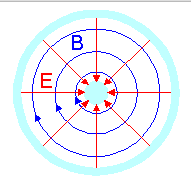
\includegraphics[scale=0.8]{22_1}$  \quad \quad \quad    $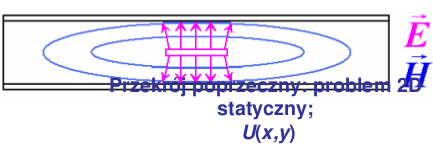
\includegraphics[scale=0.8]{22_2}$\\
	\caption{Linia współosiowa}       \qquad \qquad \qquad  \caption{Linia symetryczna paskowa}\\
%\end{floatingfigure}

%\begin{floatingfigure}
	$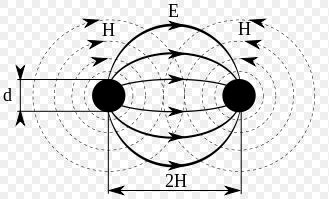
\includegraphics[scale=0.8]{22_3}$ \\
	\caption{Linia dwuprzewodowa symetryczna}\\
%\end{floatingfigure}\\
\textbf{Cechy charakterystyczne:}\\
poziom impedancji charakterystycznej: $Z_{c}=\cfrac{Z}{2\pi}\ln{\cfrac{a}{b}}$, w praktyce stosujemy linie współosiowe o impedancji od 30 $\Omega$ do 100 $\Omega$, najczęściej 50 $\Omega$.\\ 
\textbf{Cechy linii współosiowej:}
\begin{itemize}
\item dobre ekranowanie od pól zewnętrznych (na zewnątrz linii pole elektromagnetyczne jest równe zeru)
\item ograniczony zakres impedancji charakterystycznych
\item trudno robić rozgałęzienia oraz odcinki linii sprzężonych
\item trudności z dołączeniem elementów skupionych
\end{itemize}
Typowe zakresy częstotliwości: kilkadziesiąt $MHz$ do kilku $GHz$. Czasami stosowana do niskich częstotliwości. Wynika to z faktu, że pola przesyłanej fali, dla tej linii, są dobrze odizolowane od pól zewnętrznych, a więc fala ta nie jest zakłócana z zewnątrz ani też nie zakłóca innych fal rozchodzących się w pobliżu.\\
\textbf{Cechy symetrycznej linii paskowej:}\\
Znaczne ułatwienie w budowaniu rozgałęzień i linii sprzężonych w stosunku do linii współosiowej. Stosowana między innymi do budowy filtrów i sprzęgaczy falowych.\\
Przy odpowiednio szerokich płytkach ekranujących (górnej i dolnej o jednakowym potencjale) możemy uznać, że pole, podobnie jak w linii współosiowe jest zamknięte wewnątrz linii, a więc dobrze odseparowane od otoczenia.\\
\textbf{Cechy symetrycznej linii dwuprzewodowej:}\\
Linia ta znajduje zastosowanie w energetyce. Stosuje się ją w zakresie wielkich częstotliwości. Wadą tej linii jest rozproszenie pola na zewnątrz, a więc możliwość sprzężeń przesyłanego sygnału z innymi sygnałami elektronicznymi.

Zalety:
\begin{itemize}
\item prostota budowy
\item możliwość realizowania linii o dużej impredancji charakterystycznej (rzędu kilkuset $\Omega$)
\end{itemize}
Taka linia jest stosowania do połączeń odbiorników telewizyjnych z antenami.\\

\textbf{Obliczanie pojemności przewodu:}\\
$$C_{1}=\cfrac{2\pi\epsilon_{0}}{\ln{\cfrac{a}{b}}}$$
$$Z_{c}=\cfrac{Z_{0}}{2\pi}\ln{\cfrac{a}{b}} \ \ \ \ \ \ \ln{\cfrac{a}{b}}=\cfrac{Z_{c}}{Z_{0}}2\pi$$
$$C_{1}=\cfrac{Z_{0}\epsilon_{0}}{Z_{c}}=\cfrac{1}{15} \cfrac{nF}{m}$$


\end{solution}
